The following chapter gives an overview of state of the art. To achieve the high interactivity and responsiveness in the graphical discussion system, a lot of modern web technologies should be applied.

However, there are always plenty of alternatives for each technology which could differ from system to system. So it is important to investigate and analyse the existing solutions and capture an overview about different alternatives of technologies. It's is also vital to understand the benifit and drawback of the technologies used. In addition, a

First of all, the general modern web technology and development workflow will be introduced, which goes through our whole development and has a great impact on the development efficiency. The next part describes the different graphical technologies on web, and which fits our system best. Then an overview of the real time communication technologies is illustrated and evaluated. At last, a collection of modern technologies applied within the backdend server is listed.

\section{Modern Web Development}
% \section{Seperation of Frontend and Backend}


\subsection{Evolution}
With the increasing complexity of a web app and high demand of agile development, people are always thinking about how to improve patterns of the workflow in web development as well as the architecture of a web app. To achieve better scalability, maintainability and ubiquity of a web app, the architecture of an entire web app has been envolving in the past several years .

\subsubsection{Early Age}
At the early age of web development, the backend did all jobs for both client side(browser) and server side, such as rendering, calling system service, composing data, etc. Figure \ref{fig:3.1} shows the overview of web architecture:
\begin{figure}[!htbp]
  \caption{Web architecture in early age}
  \centering
    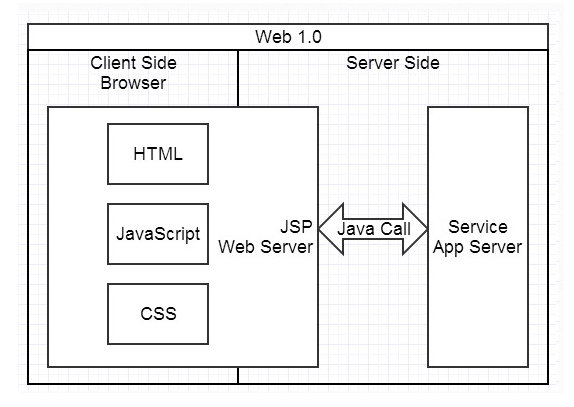
\includegraphics[width=1\textwidth]{Figures/3_1.png}
  \label{fig:3.1}
\end{figure}
The advantage of this pattern is clear: The development and deployment are simple and straightforward, if the bussiness logic doesn't become complexer. But with the increasing complexity of the product, the problems shows up:
\begin{enumerate}
\item
Development of frontend heavily depends on the whore development environment. Developers have to start up all the tools and services for testing and debugging only some small changes on view. In most cases, the frontend developer who isn't familar with the backend needs help while intergrating the new views into the system. Not only the efficiency of development, but also the cost of communication between frontend developer and backend developer are huge problems.
\item
The own responsibility of front-end and back-end mess up, which could be expressed by the commingled codes from different layers, for example there is no clear boundry from data processing tp data representing. The maintainability of the project becomes worse and worse with the increasing complexity.
\end{enumerate}

It's really significant to improve the maintainability of code, as well as the efficiency and resrationality of division of work from both front-end and back-end in the whole web development phase. In the section below, a evolution of the technical architecture will reveal how these problems are solved.

\subsubsection{Web 2.0}
Along with the birth of Gmail\footnote{https://mail.google.com/} in 2004, which is noted for its pioneering use of \gls{Ajax}, the web application started to behave more interactively. Browser began to take over the job of data fetching, processing, rendering, such a sequence of workflow which could only be done by the server side formerly.

The architecture in Web 2.0 generation is presented in figure \ref{fig:3.2}.

\begin{figure}[!htbp]
  \caption{Web 2.0 architecture}
  \centering
    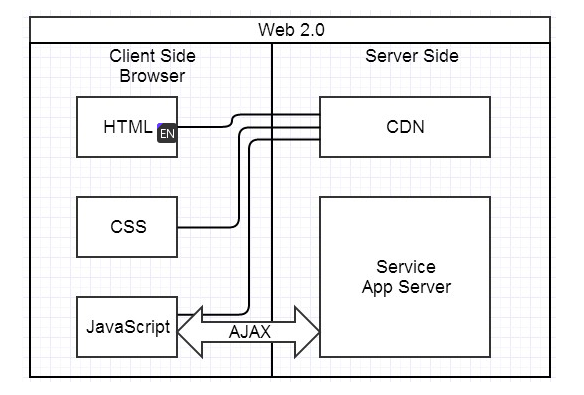
\includegraphics[width=1\textwidth]{Figures/3_2.png}
  \label{fig:3.2}
\end{figure}

By using Ajax, the client has the ability to fetching data stream asynchronously, after which the client will consume the data and render it into the specific section of view. Usability was dramatically improved, because the entired view represented to users will not be refreshed and the front-end is able to process and render data in its own intension, which means more flexible control of the consumption of data.

\subsubsection{Single Page App}

With the evolution of web technologies and promotion of these technologies in modern browswers by brower vendors, a new web development model called \gls{SPA} was proposed and caught the developers' eye. The back-end is no more responsible for rendering and view controling, it only take charge of providing services for the front-end.

\begin{figure}[!htbp]
  \caption{SPA architecture}
  \centering
    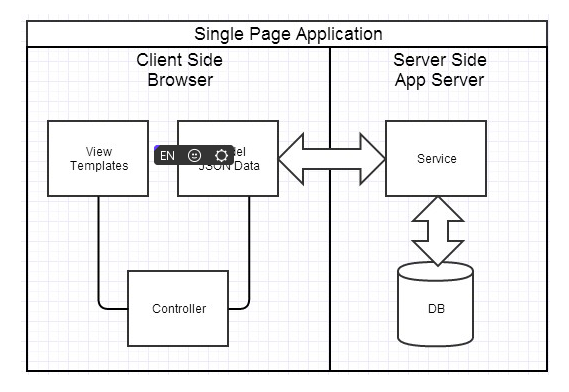
\includegraphics[width=1\textwidth]{Figures/3_3.png}
  \label{fig:3.3}
\end{figure}

The structure in figure \ref{fig:3.3} shows that the client side has the full control of view rendering and data consumption after data acquisition through web services which is released by back-end with promised protocol. All rendering tasks was stripped off from the server side, which means that the server side achieves more efficiency and concentrate more on the core bussiness logics.

But more responsibility in front-end means more complexity. How to reduce the complexity and increace the maintainability of a front-end project becomes a significant problem. Developers come up with an new envolved variant of SPA as demonstrated in figure \ref{fig:3.4}.

\begin{figure}[!htbp]
  \caption{Components in SPA}
  \centering
    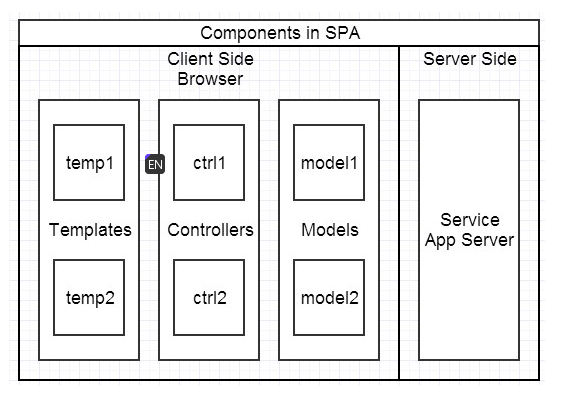
\includegraphics[width=1\textwidth]{Figures/3_4.png}
  \label{fig:3.4}
\end{figure}

In general, the architecture is componentized and layered into template, controller and model. Each component is isolated and has its own view as well as correlated logics. Front-end frameworks like EmberJS, AngularJS, ReactJS are providing such a approach and development pattern for developers to build modern web apps. With this approach, a giant and complex front-end app is broken up into fine grained components, therefore, components are easy to reuse if the components are well abstrated in a proper way. In addition, the maintaince of each component is also effortless.


\subsubsection{Trade-off}
In summarize, a single-page app has a lot of benefits:
\begin{enumerate}
\item
\textbf{Rational seperation of works from front-end and back-end}: client takes charge of view rendering and data representation, as well as slight data processing if needed; the server focus on providing services of the core logics, persistance of data, and also computational tasks.
\item
\textbf{High interactivity and user experience in client side}: asynchronous data fetching and view rendering implies no more need of hard reloading the page which user is viewing and the current states of the page could also be preserved.
\item
\textbf{Efficiency in server side}: rendering tasks are stripped off from server side.
\item
\textbf{Ubiquity}: with the seperation of services provided by server side, not only the web browser but also other clients in other platforms such as Android, iOS apps are able to access and comsume the services.
\end{enumerate}

But SPA also has its deficiencies:

\begin{enumerate}
\item
\textbf{\gls{SEO} unfriendly}: because the page are not directly rendered by server side, and the web crawlers are not able to run JavaScript codes like a browser does, the site could not be crawled properly under normal circumstances. So if SEO results really matter for the app, SPA is obviously not the best choice.
\item
\textbf{Excessive http connections}: all the data is acquired from different services through diversed \gls{API}s, thus multiple HTTP connections are established and performed parallelly, whose initial time of connections for partial data could be much more than a single connection in the traditional way. So it's highly needed to merge the services and find a balance between data model complexity and time consumption.
\end{enumerate}


\subsection{RESTful Interface}

REST is a simple way to organize interactions between independent systems. It's been growing in popularity since 2005, and inspires the design of services, such as the Twitter API. This is due to the fact that REST allows you to interact with minimal overhead with clients as diverse as mobile phones and other websites. In theory, REST is not tied to the web, but it's almost always implemented as such, and was inspired by HTTP. As a result, REST can be used wherever HTTP can.

The alternative is building relatively complex conventions on top of HTTP. Often, this takes the shape of entire new XML-based languages. The most illustrious example is SOAP. You have to learn a completely new set of conventions, but you never use HTTP to its fullest power. Because REST has been inspired by HTTP and plays to its strengths, it is the best way to learn how HTTP works.

\subsubsection{URLs}
URLs are how you identify the things that you want to operate on. We say that each URL identifies a resource. These are exactly the same URLs which are assigned to web pages. In fact, a web page is a type of resource. Let's take a more exotic example, and consider our sample application, which manages the list of a company's clients:

\begin{itemize}
  \item /clients: will identify all clients
  \item /clients/jim: will identify the client, named 'Jim', assuming that he is the only one with that name.
\end{itemize}



In these examples, we do not generally include the hostname in the URL, as it is irrelevant from the standpoint of how the interface is organized. Nevertheless, the hostname is important to ensure that the resource identifier is unique all over the web. We often say you send the request for a resource to a host. 

Finally, URLs should be as precise as needed; everything needed to uniquely identify a resource should be in the URL. You should not need to include data identifying the resource in the request. This way, URLs act as a complete map of all the data your application handles.

\subsubsection{HTTP Verbs}

HTTP verbs tell the server what to do with the data identified by the URL. The request can optionally contain additional information in its body, which might be required to perform the operation - for instance, data you want to store with the resource.

If you've ever created HTML forms, you'll be familiar with two of the most important HTTP verbs: GET and POST. But there are far more HTTP verbs available. The most important ones for building RESTful API are GET, POST, PUT and DELETE. Other methods are available, such as HEAD and OPTIONS, but they are more rare (if you want to know about all other HTTP methods, the official source is IETF).



% \subsection{Continuous Integration}



% \subsection{Operating-system-level virtualization}

% Seperation of Frontend and Backend,
\section{Graphics on the Web}
% Canvas和SVG是HTML5中主要的2D图形技术,前者提供画布标签和绘制API,后者是一整套独立的矢量图形语言,成为W3C标准已经有十多年(2003.1至今),总的来说,Canvas技术较新,从很小众发展到广泛接受,注重栅格图像处理,SVG则历史悠久,很早就成为国际标准,复杂,发展缓慢(Adobe SVG Viewer近十年没有大的更新)

% https://segmentfault.com/a/1190000000490137


% http://stackoverflow.com/questions/5882716/html5-canvas-vs-svg-vs-div


% http://smus.com/canvas-vs-svg-performance/


\subsection{Canvas}

Canvas, which is added in HTML5 as a standard, is an element defined in HTML code with width and height attributes. Graphics can be drawn on Canvas by using HTML5 Canvas APIs via scripting in JavaScript. A full set of drawing functions and helper functions could be used for accessing or rendering pixels on the Canvas area, which also means graphics can be generated dynamically and programmatically. 

Every HTML5 canvas element must have a context. All HTML5 Canvas API to be used are defined within the context. There exits two different types of context in Canvas: 2d context  for drawing 2D graphic and 3d context for 3D graphics. The latter is actually called WebGL and it’s based on OpenGL ES.

The coordinate system of Canvas set the origin offset at the upper-left corner of the canvas, with X coordinates increasing to the right and Y coordinates increasing toward the bottom of the canvas. Which means, the Canvas space doesn’t have points with negative coordinates. 

The significant features of Canvas are listed as follows:

\begin{itemize}
  \item \textbf{Interactivity}: Listeners for keyboard, mouse or touch event are able to be created in the context of Canvas. Users' actions can be captured and response will be made according to the action. 
  \item \textbf{Flexibility}: A variety of shapes like line, rectangle, circle or even text are able to be painted on the Canvas using the native methods. It is also possible to add animations, even video or audio could to the Canvas.
  \item \textbf{Browser/Platform Support}: Unlike Other graphic technology like Flash or Silverlight, which has a very restricted platform support, Canvas is supported by all major browsers which follows the HTML5 standard. In addition, it can be accessed on mobile devices via browser environment.
  \item \textbf{Performance}: Rendering pixels on Canvas is much faster comparing to other graphic technologies on Web\cite{corcoran2011effective}.
\end{itemize}


\subsection{SVG}

SVG is an XML language, similar to XHTML, which can be used to draw graphics, such as the ones shown to the right. It can be used to create an image either by specifying all the lines and shapes necessary, by modifying already existing raster images, or by a combination of both. The image and its components can also be transformed, composited together, or filtered to change their appearance completely\cite{SVGintro}.

Similar with HTML, which provides various elements for defining different styles, SVG provides elements for circles, rectangles, and simple and complex curves. A simple SVG document consists of one \textit{<svg>} element as its root element and several children elements of basic shapes. The composition of elements in SVG builds the graphic. The code listing \ref{list:svg-example-tech} shows a simple example of a SVG element with one rectangle, one circle and a text inside it.

\begin{lstlisting}[language=HTML, caption=Simple Example of SVG elemnt, label={list:svg-example-tech}]
<svg width="300" height="200" >
  <rect width="100%" height="100%" fill="red" />
  <circle cx="150" cy="100" r="80" fill="green" />
  <text x="150" y="125" font-size="60" fill="white">SVG</text>
</svg>
\end{lstlisting}


SVG is natively supported in all modern browsers and also has a good compatibility with old broswers. 

\subsection{Comparision}

\subsubsection{References to already drawn elements}
Since HTML5 Canvas is simply a drawing surface for a bit-map and renders the graphics pixel by pixel, Canvas has no knowledge of the graphics it drew: It doesn’t persist any information of the graphics' properties such as shape, position or size after the graphics were successfully drawn.

On the other hand, SVG maintains references to each object that it renders. Because each SVG element are created and appears in real DOM element on HTML. By default this allows tracking the SVG elements easily and manipulating the every existing element, for example, changing the size of an element or moving the element to another position.

\subsubsection{Rendering Performance}
Those SVG DOM references mean that some of the footwork of dealing with the things you draw is done for you. And SVG is faster when rendering really large objects, but slower when rendering many objects.

A game would probably be faster in Canvas. A huge map program would probably be faster in SVG. If you do want to use Canvas, I have some tutorials on getting movable objects up and running here.

Canvas would be better for faster things and heavy bitmap manipulation (like animation), but will take more code if you want lots of interactivity.

I've run a bunch of numbers on HTML DIV-made drawing versus Canvas-made drawing. I could make a huge post about the benefits of each, but I will give some of the relevant results of my tests to consider for your specific application:

I made Canvas and HTML DIV test pages, both had movable "nodes." Canvas nodes were objects I created and kept track of in Javascript. HTML nodes were movable Divs.

I added 100,000 nodes to each of my two tests. They performed quite differently:

The HTML test tab took forever to load (timed at slightly under 5 minutes, chrome asked to kill the page the first time). Chrome's task manager says that tab is taking up 168MB. It takes up 12-13\% CPU time when I am looking at it, 0% when I am not looking.

The Canvas tab loaded in one second and takes up 30MB. It also takes up 13\% of CPU time all of the time, regardless of whether or not one is looking at it. (2013 edit: They've mostly fixed that)

Dragging on the HTML page is smoother, which is expected by the design, since the current setup is to redraw EVERYTHING every 30 milliseconds in the Canvas test. There are plenty of optimizations to be had for Canvas for this. (canvas invalidation being the easiest, also clipping regions, selective redrawing, etc.. just depends on how much you feel like implementing)

There is no doubt you could get Canvas to be faster at object manipulation as the divs in that simple test, and of course far faster in the load time. Drawing/loading is faster in Canvas and has far more room for optimizations, too (ie, excluding things that are off-screen is very easy).
% Graphics technologies on the web
\section{Real-Time Communication}
% http://stackoverflow.com/questions/10028770/in-what-situations-would-ajax-long-short-polling-be-preferred-over-html5-websock

% HISTORY? BEFORE HTML5

% Short-Polling, Long-Polling
% WebSocket
% WebRTC


\subsection{Long polling}
HTTP Long-polling is a technique used to push updates from server to client. Establishing a connection to server using long polling is like AJAX, but the difference is that the keep-alive connection opens for a certain time period. During the connection persisted, client can retrieve data from the server connected. In case that the connection is closed or timeout unexpectedly, client have to keep requesting periodically in order to reconnect to the Server. On the server side, long polling requests are still treated as HTTP requests same as AJAX. 

Since long polling only uses normal HTTP requests, it is supported in all major browsers.


\subsection{WebSockets}

WebSockets is an advanced technology that provides the possibility to open an interactive communication session between client and server\cite{Websocket}. With the WebSockets API, messages are able to be transmitted to a server and event-driven responses can be returned to client without having to poll the server for a reply.

Starting a WebSockets connection will create TCP connection to server firstly, and keep it as long as needed. The connection can be easily closed by either by server or by client. After the HTTP compatible handshake process has succeeded,  data could be exchanged bi-directionally between server and client. Therefore, WebSockets is suitable for the heavy requirements on frequent data exchange bi-directionally. In addition, message sent through WebSockets is simply encrypted\cite{pimentel2012communicating}.


\subsection{WebRTC}

WebRTC is an industry and standards effort to put real-time capabilities into browser to browser communication and make these capabilities accessible to web developers via standard HTML5 tags and JavaScript APIs\cite{johnston2012webrtc}. 
WebRTC is used to enable the communication between multiple clients. By design, WebRTC allows to transport data in reliable as well as unreliable ways. This is generally used for high volume data transfer such as video/audio streaming where reliability is secondary and few frames or reduction in quality progression can be sacrificed in favour of response time. Both sides (peers) are able to push data to each other independently.

\subsection{Advantages}

The primary advantage of WebSockets is that the connection is not normal HTTP request, but proper message based communication protocol. That allows you to achieve huge performance and architecture advantages. Comparing to long polling, there is no need to start connection mutiple times while using WebSockets. Since the time consumption of establishing a connection is the major part of the total time consumption of a request, reducing the connection numbers will significantly improve the performance and efficiency. 

However, WebRTC is only used for peer to peer connection, but not client to server. Therefore, it is out of the scope of this thesis in general.
% Realtime technologies, comparation of techs
\section{Efficient Client Side}
\subsection{Ember.js}

Ember.js is a popular framework that utilizes a MVC framework composed of views in the form of handlebars templates. In this section, note that there is a bit of work to do in order to facilitate the integration of the templates, models, and controllers. This is not to say that Ember.js is a bad framework, because modification is a byproduct of such a framework.

In Listing 1-1, which is the body of the TodoMVC Ember.js example, you see that the markup consists of two handlebars templates for the to-do list and the to-dos.

Along with these there are three controllers—an app.js entry point, a router,
and a todo input view component. That seems like a lot of files, but in a production environment, that would be minimized. Note the separation of the controllers and views. The views, including the to-do list view shown in Listing 1-2, are quite verbose and make it easy to determine what the code does.


This is a clear example and works as a readable view. There are several properties that are dictated from the controller as you would expect. The controller is named in the router.js file, which also names the view to be used. This controller is shown in the Listing 1-3.

You can see that this TodosListController takes a model of to-dos and adds some properties along with the itemController of 'todo'. This todo controller is actually where most of the JavaScript resides that dictates the actions and conditionals that are visible in the view you saw earlier in this section. As someone who is familiar with Ember. js, this is a well defined and organized example of what Ember.js can do. It is however quite different than React, which you will see soon enough. First, let’s examine a bit of the AngularJS TodoMVC example.

\subsection{AngularJS}

AngularJS is perhaps the world’s most popular MV* framework. It is extremely simple to get started and has the backing of Google along with many developers who have jumped in and created great tutorials, books, and blog posts. It is of course not the same framework as React, which you will soon see. Listing 1-4 shows the AngularJS TodoMVC application.

You can see already that compared to Ember.js, Angular is more declarative in nature in its templating. You can also see that there are concepts like controllers, directives, and services that are tied to this application. The todoCtrl file holds the controller values that power this view. The next example, shown in Listing 1-5, is just a snippet of this file, but you can see how it works.


This example showcases the todoCtrl and shows how it builds a \$scope mechanism that then allows you to attach methods and properties to your AngularJS view. The next section dives into React and explains how it acts on a user interface in a different way than Ember.js and AngularJS do.


\subsection{React}

As you saw in the other examples, there is a basic structure to the TodoMVC applications that makes them an easy choice for demonstrating differences. Ember.js and AngularJS are two popular frameworks that I think help demonstrate that React is not an MV* framework and just a basic JavaScript framework for building user interfaces. This section details the React example and shows you how to structure a React app from the component level, and then works backward to explain how the components are composed. And now, many pages into a book about React, you finally get to see React code in Listing 1-6.

In this example, you see the rendering of the TodoItem component, which is a
subcomponent of the TodoApp. This is simply a component that handles the individual list 14

items that are contained in the TodoApp. This is split off into its own component because
it represents its own set of interactions in the application. It can handle editing as well as marking if the item is completed or not. Since this functionality doesn’t necessarily need to know or interact with the rest of the application, it is built as a standalone component. It may have been just as easy to add to the TodoApp itself initially, but in the world of React, as you will see later, it is often better to make things more modular. This is because in the future the maintenance costs will be recouped by utilizing this logical separation of interactions.
Now you understand at a high level how interactions can often be contained in subcomponents in a React application. The code of the TodoApp render function shows that the TodoItem exists as a subcomponent and shows that the TodoFooter, contained in a JSX by itself, houses its own interactions. The next important concept is to focus on how these subcomponents are reassembled. The TodoItems are added to an unordered list that is contained in a variable called main, which returns the JSX markup for the main section of the TodoApp. Similarly the footer variable contains the TodoFooter component. These two variables, footer and main, are added to the return value of the TodoApp, which you see at the end of the example. These variables are accessed in JSX by using curly braces so you see them as follows:


\subsection{Why React.js}

In many cases when you learn something, you first need to realize what the thing is that you are learning. In the case of React, it can be helpful to learn which concepts are not parts of the React framework. This will help you understand which standard practices you have learned need to be unlearned, or at least need to be set aside, in order to fully understand the concepts of a new framework such as React. So what is it that makes React different and why is it important?

Many argue that React is a full-scale JavaScript framework on a level that compares to other frameworks such as Backbone, Knockout.js, AngularJS, Ember, CanJS, Dojo, or any of the numerous MVC frameworks that exist. Figure 1-1 shows an example of a typical MVC framework.

Figure 1-1 shows the basics of each of the components in a Model-View-Controller architecture. The model handles the state of the application and sends state-changing events to the view. The view is the user-facing look and interaction interface to the end user. The view can send events to the controller, and in some cases to the model. The controller is the main dispatcher of events, which can be sent to the model, to update state, and the view to update the presentation. You may note that this is a generic representation of what an MVC architecture is, and in reality there are so many variants and customized implementations that there is no single MVC architecture. The point isn’t to state what an MVC structure looks like, but to point out what React is not.

This MVC structure is actually not a fair assessment of what React is or intends to be. That is because React is one particular piece of what these frameworks present. React is in its simplest form, just the view of these MVC, MVVM, or MV* frameworks. As you saw in the previous section, React is a way to describe the user interface of an application and a mechanism to change that over time as data changes. React is made with declarative components that describe an interface. React uses no observable data binding when building an application. React is also easy to manipulate, because you can take the components you create and combine them to make custom components that work as you expect every time because it can scale. React can scale better than other frameworks because of the principles that drove it from its creation. When creating React interfaces, you structure them in such as way that they are built out of multiple components.

Let’s pause for a minute and examine the most basic structure of several frameworks and then compare them to React in order to highlight the differences. For each of the frameworks, you will examine the most basic to-do list applications as they are created for the http://todomvc.com web site. I am not going to deride other frameworks because they all serve a purpose. Instead I attempt to demonstrate how React is structured compared to the others. I showcase just the important parts to highlight and limit a complete recreation of the application here. If you want to see the full examples, the links to the source are included. Try not to become too focused on the implementation details of any of these examples, including the React example, because as you progress through this book the concepts will be covered thoroughly and will help you understand what is going on completely.
% Tech stack: React, Babel, ES6, ...
\section{Efficient Server Side}
This section gives the explanation of architectural pattern and more detailed implementation of the server side. 

% Architecture MV, , JWT for Auth, Websocket Dispatcher, Resource Listening?

\subsection{Architecture}

\subsubsection{MVC Pattern and Project Structure}
To separate the different layers of model, view and controller, \gls{MVC} pattern is used as the basic pattern of the architecture. In the model layer, all data model related concerns such as data shema definitions, data model validation as well as database operations are defined. And Controllers contain the core domain logics, process the data from model layer, and pass the result to view layer.

Since the templates are rendered on the client side, the view layer is just simply stripped. Therefore, basically the controllers response processed data to client side directly without rendering it to views. Figure \ref{fig:server-file-structure-imp} shows the overview of the server's  file structure which is featured with MVC pattern.

\begin{figure}[!htbp]
\centering
\begin{forest}
  for tree={
    font=\ttfamily,
    grow'=0,
    child anchor=west,
    parent anchor=south,
    anchor=west,
    calign=first,
    edge path={
      \noexpand\path [draw, \forestoption{edge}]
      (!u.south west) +(7.5pt,0) |- node[fill,inner sep=1.25pt] {} (.child anchor)\forestoption{edge label};
    },
    before typesetting nodes={
      if n=1
        {insert before={[,phantom]}}
        {}
    },
    fit=band,
    before computing xy={l=15pt},
  }
[server
  [config/
    [index.js]
    [routes.js]
  ]
  [models/]
  [controllers/]
  [index.js]
  [...]
]
\end{forest}
\caption{Overview of server app's file structure}
\label{fig:server-file-structure-imp}
\end{figure}


\begin{enumerate}
\item 
  \textbf{index.js}: the entry point of the whole server app. It will create a server instance and set up configurations for the server. In addition, a connection from server instance to database will be established. After all configurations are done, the server instance will start listening port and waiting for the requests from client.
\item
  \textbf{config/index.js}: config as well as constants for the server. It persists \textit{apiConfig} for example the common prefix of API URL and version of the API. And config for database including the database URL will be defined here as well. In addition, keys for encryption are also stored in the config file.
\item
  \textbf{config/routes.js}: rules for URL matching. All URL matching rules are defined in this file. Controllers are referenced here and a dispatcher for router will be instantiated. If any request meets the defined rule, the request will be forward to a correlative controller. 
\item
  \textbf{controllers/*}: controllers for processing specific requests.
\item 
  \textbf{models/*}: data model definitions. Files under this directory are organized by different data domain.
\end{enumerate}


\subsubsection{Achitecture of Server}

The figure \ref{fig:server-arch-imp} illustrates an overview of the server's architecture. 

\begin{figure}[!htbp]
  \centering
    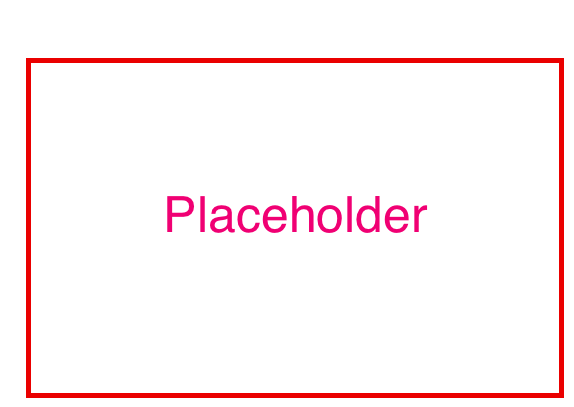
\includegraphics[width=0.6\textwidth]{Figures/placeholder.png}
  \caption{placeholder}
  \label{fig:server-arch-imp}
\end{figure}
% process of request to be handeled. index.js -> create server isntance -> connect to database. routes -> different controllers -> different models

\subsection{Data Schema Definition}
% Tech stack: Nodejs (Why Node, comparation), MongoDB(Why, comparaion), Express?


\section{Conclusion}

TBD